\section{Deduplication Analysis}
\label{sec:dedup}

\subsection{File level deduplication ratio}

\subsubsection{Redundant file overhead in terms of file repeat count and redundant storage overhead}

\paragraph{File repeat count distribution.}

\begin{figure}
	\centering
	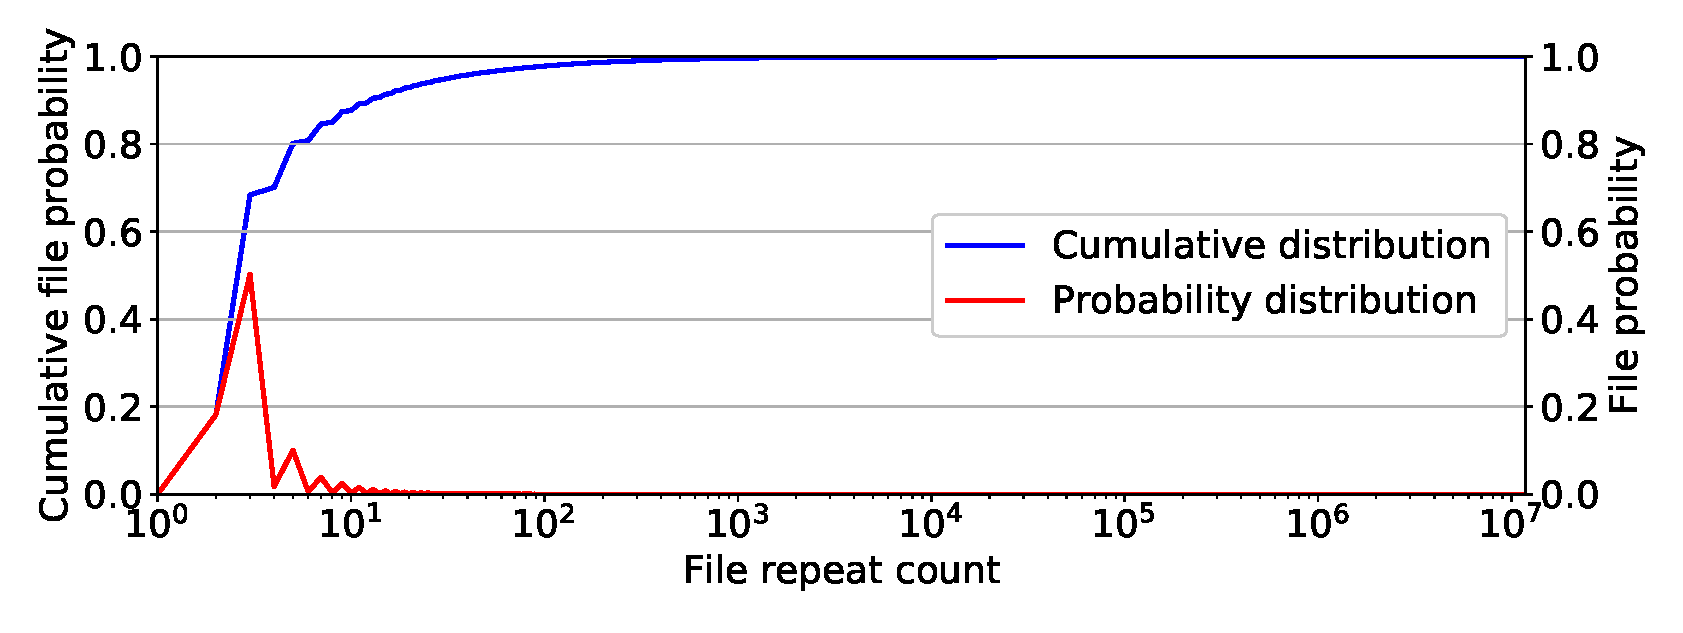
\includegraphics[width=0.5\textwidth]{graphs/File_repeat_count.eps}
	\caption{CDF of file repeat count.
	}
	\label{fig_file_repeat_count}
\end{figure}

\paragraph{Unique file size distribution.}

\begin{figure}
	\centering
	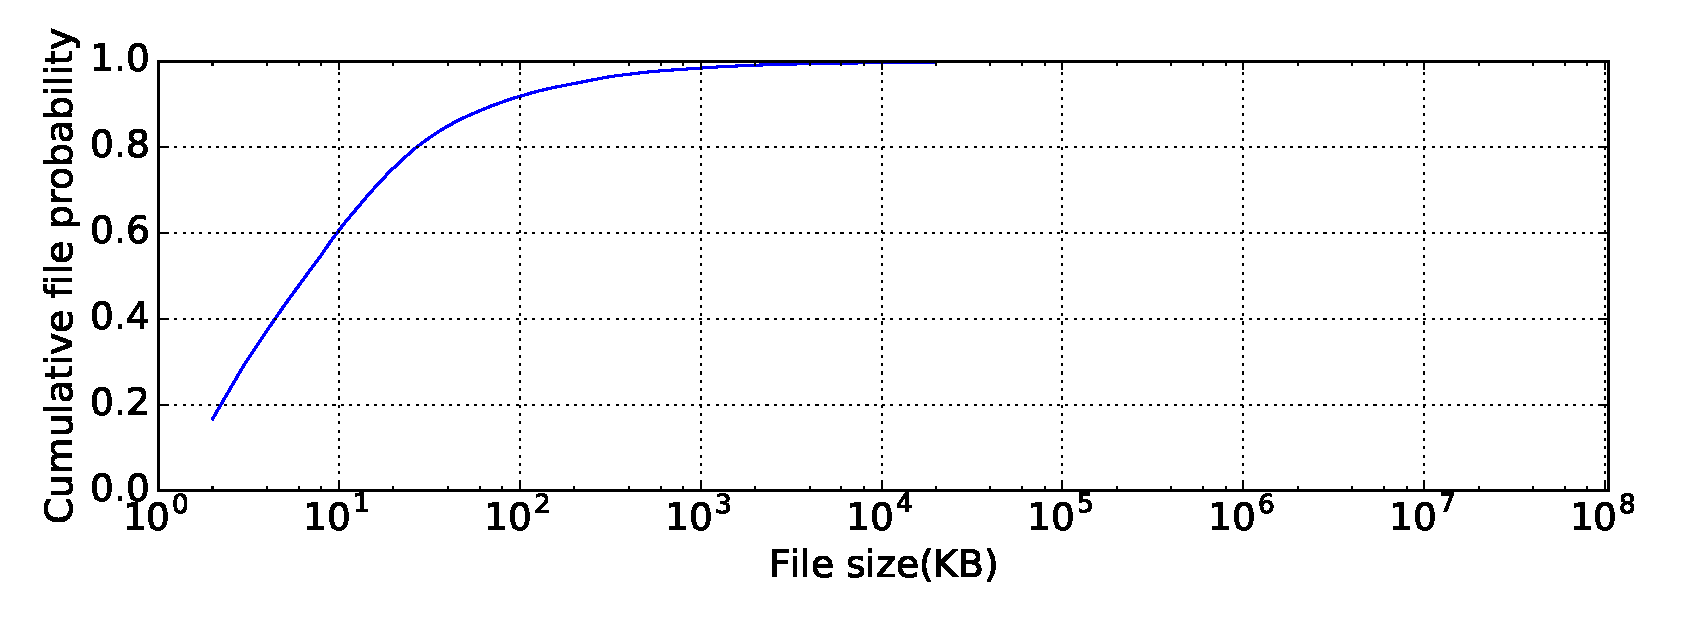
\includegraphics[width=0.5\textwidth]{graphs/File_size-KB.eps}
	\caption{CDF of unique file size.
	}
	\label{fig_file_size}
\end{figure}

\paragraph{Redundant file storage overhead.}

\begin{figure}
	\centering
	\includegraphics[width=0.5\textwidth]{graphs/Total_size_of_redudant_files_with_same_content-KB.eps}
	\caption{CDF of total file size with same file content.
	}
	\label{fig_redundant_size}
\end{figure}

\paragraph{Average file size by repeat count.}


\paragraph{Total file size by repeat count.}


\subsubsection{What are the redundant files?}


\subsection{Suggest 1: File-Level Content Addressable Storage Model}


\subsection{Redundant files in layers}


\subsubsection{Redundant storage overhead for individual layers}


\subsubsection{Redundant storage overhead across layers}


\subsubsection{Why do layers have so many redundant files?}


\subsection{Redundant files in images}

%\subsubsection{Redundant file characterization}

\subsection{Chunking Deduplication}

\subsubsection{Chunking Deduplication ratio}
